% Preview of the new sections before the restructure: python paper/make_numbers.py, then build this file from paper/.
\documentclass[conference]{IEEEtran}
\usepackage[T1]{fontenc}
\usepackage{cite}
\usepackage{amsmath,amssymb,amsfonts}
\usepackage{graphicx}
\usepackage{textcomp}
\usepackage{xcolor}
\usepackage{booktabs}
\usepackage{pifont}
\usepackage[hidelinks]{hyperref}
\usepackage{xurl}
\usepackage{tikz}
\usetikzlibrary{positioning,arrows.meta,fit,shapes.geometric}
% Generated by paper/make_numbers.py from results/; do not edit by hand.
\newcommand{\CensusSample}{2{,}000}  % results/census/phase2/rq1.json
\newcommand{\DriftPkgs}{731/2{,}000}  % results/census/phase2/rq1.json
\newcommand{\DriftPkgsP}{36.5\%}  % results/census/phase2/rq1.json
\newcommand{\DriftPkgsCI}{[34.5, 38.7]}  % results/census/phase2/rq1.json
\newcommand{\DriftWinRel}{731/1{,}239}  % results/census/phase2/rq1.json
\newcommand{\DriftWinRelP}{59.0\%}  % results/census/phase2/rq1.json
\newcommand{\DriftWinRelCI}{[56.2, 61.7]}  % results/census/phase2/rq1.json
\newcommand{\DriftTrans}{2{,}259/6{,}695}  % results/census/phase2/rq1.json
\newcommand{\DriftTransP}{33.7\%}  % results/census/phase2/rq1.json
\newcommand{\DriftTransCI}{[32.6, 34.9]}  % results/census/phase2/rq1.json
\newcommand{\Extractable}{9{,}994/12{,}768}  % results/census/phase2/rq1.json
\newcommand{\ExtractableP}{78.3\%}  % results/census/phase2/rq1.json
\newcommand{\ExtractableCI}{[77.6, 79.0]}  % results/census/phase2/rq1.json
\newcommand{\NoSignal}{2{,}192/2{,}259}  % results/census/phase2/rq1.json
\newcommand{\NoSignalP}{97.0\%}  % results/census/phase2/rq1.json
\newcommand{\NoSignalCI}{[96.3, 97.7]}  % results/census/phase2/rq1.json
\newcommand{\CoSignalMinP}{0.25}  % results/census/phase2/rq1.json
\newcommand{\KindAdded}{987}  % results/census/phase2/rq1.json
\newcommand{\KindRemoved}{132}  % results/census/phase2/rq1.json
\newcommand{\KindDesc}{1{,}374}  % results/census/phase2/rq1.json
\newcommand{\KindSchema}{1{,}157}  % results/census/phase2/rq1.json
\newcommand{\ValN}{82}  % results/census/phase2/validation_heldout_summary.json
\newcommand{\ValPrec}{92.2\%}  % results/census/phase2/validation_heldout_summary.json
\newcommand{\ValRec}{78.0\%}  % results/census/phase2/validation_heldout_summary.json
\newcommand{\MetaPkgs}{15{,}272}  % results/census/metacensus/summary.json
\newcommand{\MetaTrans}{228{,}044}  % results/census/metacensus/summary.json
\newcommand{\MetaNpmActive}{10{,}693}  % results/census/metacensus/summary.json
\newcommand{\MetaPyActive}{3{,}957}  % results/census/metacensus/summary.json
\newcommand{\MetaProvLostNpm}{390/10{,}693}  % results/census/metacensus/summary.json
\newcommand{\MetaProvLostNpmP}{3.65\%}  % results/census/metacensus/summary.json
\newcommand{\MetaProvLostNpmCI}{[3.31, 4.02]}  % results/census/metacensus/summary.json
\newcommand{\MetaLatestProvNpm}{2{,}898/11{,}201}  % results/census/metacensus/summary.json
\newcommand{\MetaLatestProvNpmP}{25.9\%}  % results/census/metacensus/summary.json
\newcommand{\MetaLatestProvNpmCI}{[25.1, 26.7]}  % results/census/metacensus/summary.json
\newcommand{\MetaProvLostPy}{212/3{,}957}  % results/census/metacensus/summary.json
\newcommand{\MetaProvLostPyP}{5.36\%}  % results/census/metacensus/summary.json
\newcommand{\MetaProvLostPyCI}{[4.70, 6.10]}  % results/census/metacensus/summary.json
\newcommand{\MetaLatestProvPy}{1{,}889/4{,}071}  % results/census/metacensus/summary.json
\newcommand{\MetaLatestProvPyP}{46.4\%}  % results/census/metacensus/summary.json
\newcommand{\MetaLatestProvPyCI}{[44.9, 47.9]}  % results/census/metacensus/summary.json
\newcommand{\MetaInstallNpm}{203/10{,}693}  % results/census/metacensus/summary.json
\newcommand{\MetaInstallNpmP}{1.90\%}  % results/census/metacensus/summary.json
\newcommand{\MetaInstallNpmCI}{[1.66, 2.17]}  % results/census/metacensus/summary.json
\newcommand{\MetaMaintNpm}{598/10{,}693}  % results/census/metacensus/summary.json
\newcommand{\MetaMaintNpmP}{5.59\%}  % results/census/metacensus/summary.json
\newcommand{\MetaMaintNpmCI}{[5.17, 6.04]}  % results/census/metacensus/summary.json
\newcommand{\MetaCiHuman}{241/10{,}693}  % results/census/metacensus/publisher_breakdown.json
\newcommand{\MetaCiHumanP}{2.25\%}  % results/census/metacensus/publisher_breakdown.json
\newcommand{\MetaCiHumanCI}{[1.99, 2.55]}  % results/census/metacensus/publisher_breakdown.json
\newcommand{\MetaHumanCi}{2{,}568/10{,}693}  % results/census/metacensus/publisher_breakdown.json
\newcommand{\MetaHumanCiP}{24.0\%}  % results/census/metacensus/publisher_breakdown.json
\newcommand{\MetaHumanCiCI}{[23.2, 24.8]}  % results/census/metacensus/publisher_breakdown.json
\newcommand{\NR}{490}  % results/candidate/phase4/phase4_results.json
\newcommand{\NB}{8{,}180}  % results/candidate/phase4/phase4_results.json
\newcommand{\NRM}{468}  % results/candidate/phase4/phase4_results.json
\newcommand{\NRMC}{368}  % results/candidate/phase4/phase4_results.json
\newcommand{\NRMN}{100}  % results/candidate/phase4/phase4_results.json
\newcommand{\NRB}{22}  % results/candidate/phase4/phase4_results.json
\newcommand{\DetG}{195/490}  % results/candidate/phase4/phase4_results.json
\newcommand{\DetGP}{39.8\%}  % results/candidate/phase4/phase4_results.json
\newcommand{\DetGCI}{[35.6, 44.2]}  % results/candidate/phase4/phase4_results.json
\newcommand{\DetSC}{96/490}  % results/candidate/phase4/phase4_results.json
\newcommand{\DetSCP}{19.6\%}  % results/candidate/phase4/phase4_results.json
\newcommand{\DetSCCI}{[16.3, 23.3]}  % results/candidate/phase4/phase4_results.json
\newcommand{\DetSL}{71/490}  % results/candidate/phase4/phase4_results.json
\newcommand{\DetSLP}{14.5\%}  % results/candidate/phase4/phase4_results.json
\newcommand{\DetSLCI}{[11.6, 17.9]}  % results/candidate/phase4/phase4_results.json
\newcommand{\DetGBlock}{192/490}  % results/candidate/phase4/phase4_results.json
\newcommand{\DetGBlockP}{39.2\%}  % results/candidate/phase4/phase4_results.json
\newcommand{\DetGBlockCI}{[35.0, 43.6]}  % results/candidate/phase4/phase4_results.json
\newcommand{\DetSCBlock}{96/490}  % results/candidate/phase4/phase4_results.json
\newcommand{\DetSCBlockP}{19.6\%}  % results/candidate/phase4/phase4_results.json
\newcommand{\DetSCBlockCI}{[16.3, 23.3]}  % results/candidate/phase4/phase4_results.json
\newcommand{\AddedDet}{99}  % results/candidate/phase4/phase4_results.json
\newcommand{\SCOnly}{0}  % results/candidate/phase4/phase4_results.json
\newcommand{\McNemarHOne}{3.2\times10^{-30}}  % results/candidate/phase4/phase4_results.json
\newcommand{\HolmHOne}{6.3\times10^{-30}}  % results/candidate/phase4/phase4_results.json
\newcommand{\FbG}{2{,}729/8{,}180}  % results/candidate/phase4/phase4_results.json
\newcommand{\FbGP}{33.4\%}  % results/candidate/phase4/phase4_results.json
\newcommand{\FbGCI}{[32.3, 34.4]}  % results/candidate/phase4/phase4_results.json
\newcommand{\FbSC}{2{,}695/8{,}180}  % results/candidate/phase4/phase4_results.json
\newcommand{\FbSCP}{32.9\%}  % results/candidate/phase4/phase4_results.json
\newcommand{\FbSCCI}{[31.9, 34.0]}  % results/candidate/phase4/phase4_results.json
\newcommand{\WarnG}{1{,}346/8{,}180}  % results/candidate/phase4/phase4_results.json
\newcommand{\WarnGP}{16.5\%}  % results/candidate/phase4/phase4_results.json
\newcommand{\WarnGCI}{[15.7, 17.3]}  % results/candidate/phase4/phase4_results.json
\newcommand{\InterG}{4{,}075/8{,}180}  % results/candidate/phase4/phase4_results.json
\newcommand{\InterGP}{49.8\%}  % results/candidate/phase4/phase4_results.json
\newcommand{\InterGCI}{[48.7, 50.9]}  % results/candidate/phase4/phase4_results.json
\newcommand{\FbExtra}{34}  % results/candidate/phase4/phase4_results.json
\newcommand{\FbDiffPP}{0.42}  % results/candidate/phase4/phase4_results.json
\newcommand{\FbDiffCI}{[0.28, 0.56]}  % results/candidate/phase4/phase4_results.json
\newcommand{\McNemarHTwo}{1.2\times10^{-10}}  % results/candidate/phase4/phase4_results.json
\newcommand{\AblTwo}{0}  % results/candidate/phase4/phase4_results.json
\newcommand{\AblThree}{1}  % results/candidate/phase4/phase4_results.json
\newcommand{\AblFour}{96}  % results/candidate/phase4/phase4_results.json
\newcommand{\AblFive}{2}  % results/candidate/phase4/phase4_results.json
\newcommand{\RMCG}{116/368}  % results/candidate/phase4/phase4_results.json
\newcommand{\RMCGP}{31.5\%}  % results/candidate/phase4/phase4_results.json
\newcommand{\RMCGCI}{[27.0, 36.4]}  % results/candidate/phase4/phase4_results.json
\newcommand{\RMCSC}{17/368}  % results/candidate/phase4/phase4_results.json
\newcommand{\RMCSCP}{4.6\%}  % results/candidate/phase4/phase4_results.json
\newcommand{\RMCSCCI}{[2.9, 7.3]}  % results/candidate/phase4/phase4_results.json
\newcommand{\RMNG}{59/100}  % results/candidate/phase4/phase4_results.json
\newcommand{\RMNGP}{59.0\%}  % results/candidate/phase4/phase4_results.json
\newcommand{\RMNGCI}{[49.2, 68.1]}  % results/candidate/phase4/phase4_results.json
\newcommand{\RSG}{40/40}  % results/candidate/phase4/phase4_results.json
\newcommand{\RSSC}{0/40}  % results/candidate/phase4/phase4_results.json
\newcommand{\RSCtrl}{0/10}  % results/candidate/phase4/phase4_results.json
\newcommand{\STwoB}{3{,}261/8{,}180}  % results/candidate/phase4/phase4_results.json
\newcommand{\STwoBP}{39.9\%}  % results/candidate/phase4/phase4_results.json
\newcommand{\STwoBCI}{[38.8, 40.9]}  % results/candidate/phase4/phase4_results.json
\newcommand{\STwoRMC}{50/368}  % results/candidate/phase4/phase4_results.json
\newcommand{\STwoRMCP}{13.6\%}  % results/candidate/phase4/phase4_results.json
\newcommand{\STwoRMCCI}{[10.5, 17.5]}  % results/candidate/phase4/phase4_results.json
\newcommand{\EvalSTwo}{88}  % results/candidate/phase4/phase4_results.json
\newcommand{\EvalSFour}{214}  % results/candidate/phase4/phase4_results.json
\newcommand{\EvalSFive}{239}  % results/candidate/phase4/phase4_results.json
\newcommand{\FbPerDet}{0.34}  % results/candidate/phase4/phase4_results.json
\newcommand{\WarnPerDet}{13.6}  % results/candidate/phase4/phase4_results.json
\newcommand{\LatN}{199}  % results/candidate/phase4/phase4_results.json
\newcommand{\LatColdMed}{0.99}  % results/candidate/phase4/phase4_results.json
\newcommand{\LatColdPNF}{3.19}  % results/candidate/phase4/phase4_results.json
\newcommand{\LatColdMax}{50.8}  % results/candidate/phase4/phase4_results.json
\newcommand{\LatWarmMed}{0.05}  % results/candidate/phase4/phase4_results.json
\newcommand{\NBMcp}{6{,}695}  % results/candidate/phase4/phase4_results.json
\newcommand{\NBNpmTop}{992}  % results/candidate/phase4/phase4_results.json
\newcommand{\NBPyTop}{493}  % results/candidate/phase4/phase4_results.json
\newcommand{\FbSCMcp}{2{,}683/6{,}695}  % results/candidate/phase4/phase4_results.json
\newcommand{\FbSCMcpP}{40.1\%}  % results/candidate/phase4/phase4_results.json
\newcommand{\FbSCMcpCI}{[38.9, 41.3]}  % results/candidate/phase4/phase4_results.json
\newcommand{\WarnGMcp}{1{,}321/6{,}695}  % results/candidate/phase4/phase4_results.json
\newcommand{\WarnGMcpP}{19.7\%}  % results/candidate/phase4/phase4_results.json
\newcommand{\WarnGMcpCI}{[18.8, 20.7]}  % results/candidate/phase4/phase4_results.json
\newcommand{\SensN}{88}  % results/candidate/phase4/phase4_results.json
\newcommand{\SensG}{61}  % results/candidate/phase4/phase4_results.json
\newcommand{\SensSC}{56}  % results/candidate/phase4/phase4_results.json
\newcommand{\ENCases}{12}  % results/candidate/phase5/evasion_matrix.json
\newcommand{\EGBlock}{1}  % results/candidate/phase5/evasion_matrix.json
\newcommand{\EGWarn}{4}  % results/candidate/phase5/evasion_matrix.json
\newcommand{\EGAllow}{7}  % results/candidate/phase5/evasion_matrix.json
\newcommand{\EGStop}{5}  % results/candidate/phase5/evasion_matrix.json
\newcommand{\ESCAllow}{12}  % results/candidate/phase5/evasion_matrix.json
\newcommand{\EAllBlock}{10}  % results/candidate/phase5/evasion_matrix.json
\newcommand{\EElevenN}{22}  % results/candidate/phase5/evasion_matrix.json
\newcommand{\EElevenG}{13}  % results/candidate/phase5/evasion_matrix.json
\newcommand{\EElevenH}{21}  % results/candidate/phase5/evasion_matrix.json
\newcommand{\ExpNoProv}{4{,}919/8{,}180}  % results/candidate/phase5/exposure.json
\newcommand{\ExpNoProvP}{60.1\%}  % results/candidate/phase5/exposure.json
\newcommand{\ExpNoProvCI}{[59.1, 61.2]}  % results/candidate/phase5/exposure.json
\newcommand{\ExpNonStatic}{2{,}774/12{,}768}  % results/candidate/phase5/exposure.json
\newcommand{\ExpNonStaticP}{21.7\%}  % results/candidate/phase5/exposure.json
\newcommand{\ExpNonStaticCI}{[21.0, 22.4]}  % results/candidate/phase5/exposure.json
\newcommand{\ExpFloatSdk}{1{,}027/1{,}094}  % results/candidate/phase5/exposure.json
\newcommand{\ExpFloatSdkP}{93.9\%}  % results/candidate/phase5/exposure.json
\newcommand{\ExpFloatSdkCI}{[92.3, 95.2]}  % results/candidate/phase5/exposure.json
\newcommand{\HTwoLo}{2{,}213/8{,}180}  % results/candidate/phase5/hardening_cost.json
\newcommand{\HTwoLoP}{27.1\%}  % results/candidate/phase5/hardening_cost.json
\newcommand{\HTwoLoCI}{[26.1, 28.0]}  % results/candidate/phase5/hardening_cost.json
\newcommand{\HTwoHi}{2{,}259/8{,}180}  % results/candidate/phase5/hardening_cost.json
\newcommand{\HTwoHiP}{27.6\%}  % results/candidate/phase5/hardening_cost.json
\newcommand{\HTwoHiCI}{[26.7, 28.6]}  % results/candidate/phase5/hardening_cost.json
\newcommand{\HTwoMcp}{2{,}213/6{,}695}  % results/candidate/phase5/hardening_cost.json
\newcommand{\HTwoMcpP}{33.0\%}  % results/candidate/phase5/hardening_cost.json
\newcommand{\HTwoMcpCI}{[31.9, 34.2]}  % results/candidate/phase5/hardening_cost.json
\newcommand{\HTwoUnmeas}{1{,}483}  % results/candidate/phase5/hardening_cost.json
\newcommand{\HTwoAddLo}{1{,}286/8{,}180}  % results/candidate/phase5/hardening_cost.json
\newcommand{\HTwoAddLoP}{15.7\%}  % results/candidate/phase5/hardening_cost.json
\newcommand{\HTwoAddLoCI}{[14.9, 16.5]}  % results/candidate/phase5/hardening_cost.json
\newcommand{\HTwoAddHi}{1{,}319/8{,}180}  % results/candidate/phase5/hardening_cost.json
\newcommand{\HTwoAddHiP}{16.1\%}  % results/candidate/phase5/hardening_cost.json
\newcommand{\HTwoAddHiCI}{[15.3, 16.9]}  % results/candidate/phase5/hardening_cost.json
\newcommand{\HFourAdd}{3{,}048/8{,}180}  % results/candidate/phase5/hardening_cost.json
\newcommand{\HFourAddP}{37.3\%}  % results/candidate/phase5/hardening_cost.json
\newcommand{\HFourAddCI}{[36.2, 38.3]}  % results/candidate/phase5/hardening_cost.json
\newcommand{\HThreeLate}{12/2{,}528}  % results/candidate/phase5/hardening_cost.json
\newcommand{\HThreeLateP}{0.47\%}  % results/candidate/phase5/hardening_cost.json
\newcommand{\HThreeLateCI}{[0.27, 0.83]}  % results/candidate/phase5/hardening_cost.json
\newcommand{\HThreeLateDay}{3/2{,}528}  % results/candidate/phase5/hardening_cost.json
\newcommand{\HThreeLateDayP}{0.12\%}  % results/candidate/phase5/hardening_cost.json
\newcommand{\HThreeLateDayCI}{[0.04, 0.35]}  % results/candidate/phase5/hardening_cost.json
\newcommand{\HFour}{4{,}700/8{,}180}  % results/candidate/phase5/hardening_cost.json
\newcommand{\HFourP}{57.5\%}  % results/candidate/phase5/hardening_cost.json
\newcommand{\HFourCI}{[56.4, 58.5]}  % results/candidate/phase5/hardening_cost.json
\newcommand{\HFive}{0/8{,}180}  % results/candidate/phase5/hardening_cost.json
\newcommand{\HFiveP}{0.0\%}  % results/candidate/phase5/hardening_cost.json
\newcommand{\HFiveCI}{[0.0, 0.1]}  % results/candidate/phase5/hardening_cost.json
\newcommand{\HOneN}{5{,}652}  % results/candidate/phase5/hardening_cost.json
\newcommand{\HOneBlockEarly}{58/5{,}652}  % results/candidate/phase5/hardening_cost.json
\newcommand{\HOneBlockEarlyP}{1.03\%}  % results/candidate/phase5/hardening_cost.json
\newcommand{\HOneBlockEarlyCI}{[0.79, 1.32]}  % results/candidate/phase5/hardening_cost.json
\newcommand{\HOneWarnEarly}{199/5{,}652}  % results/candidate/phase5/hardening_cost.json
\newcommand{\HOneWarnEarlyP}{3.52\%}  % results/candidate/phase5/hardening_cost.json
\newcommand{\HOneWarnEarlyCI}{[3.07, 4.03]}  % results/candidate/phase5/hardening_cost.json
\newcommand{\HOneStrictEarly}{2{,}765/5{,}652}  % results/candidate/phase5/hardening_cost.json
\newcommand{\HOneStrictEarlyP}{48.9\%}  % results/candidate/phase5/hardening_cost.json
\newcommand{\HOneStrictEarlyCI}{[47.6, 50.2]}  % results/candidate/phase5/hardening_cost.json
\newcommand{\HOneBlockLate}{30/5{,}652}  % results/candidate/phase5/hardening_cost.json
\newcommand{\HOneBlockLateP}{0.53\%}  % results/candidate/phase5/hardening_cost.json
\newcommand{\HOneBlockLateCI}{[0.37, 0.76]}  % results/candidate/phase5/hardening_cost.json
\newcommand{\HOneWarnLate}{5/5{,}652}  % results/candidate/phase5/hardening_cost.json
\newcommand{\HOneWarnLateP}{0.09\%}  % results/candidate/phase5/hardening_cost.json
\newcommand{\HOneWarnLateCI}{[0.04, 0.21]}  % results/candidate/phase5/hardening_cost.json
\newcommand{\HOneStrictLate}{698/5{,}652}  % results/candidate/phase5/hardening_cost.json
\newcommand{\HOneStrictLateP}{12.3\%}  % results/candidate/phase5/hardening_cost.json
\newcommand{\HOneStrictLateCI}{[11.5, 13.2]}  % results/candidate/phase5/hardening_cost.json
\newcommand{\HOneMedNodes}{96}  % results/candidate/phase5/hardening_cost.json
\newcommand{\HOneNewPub}{486}  % results/candidate/phase5/hardening_cost.json
\newcommand{\AgeFb}{60/8{,}180}  % results/candidate/phase5/age_rule_sensitivity.json
\newcommand{\AgeFbP}{0.73\%}  % results/candidate/phase5/age_rule_sensitivity.json
\newcommand{\AgeFbCI}{[0.57, 0.94]}  % results/candidate/phase5/age_rule_sensitivity.json
\newcommand{\AgeWarn}{2{,}264/8{,}180}  % results/candidate/phase5/age_rule_sensitivity.json
\newcommand{\AgeWarnP}{27.7\%}  % results/candidate/phase5/age_rule_sensitivity.json
\newcommand{\AgeWarnCI}{[26.7, 28.7]}  % results/candidate/phase5/age_rule_sensitivity.json
\newcommand{\AgeInter}{2{,}324/8{,}180}  % results/candidate/phase5/age_rule_sensitivity.json
\newcommand{\AgeInterP}{28.4\%}  % results/candidate/phase5/age_rule_sensitivity.json
\newcommand{\AgeInterCI}{[27.4, 29.4]}  % results/candidate/phase5/age_rule_sensitivity.json
\newcommand{\AgeDet}{187/490}  % results/candidate/phase5/age_rule_sensitivity.json
\newcommand{\AgeDetP}{38.2\%}  % results/candidate/phase5/age_rule_sensitivity.json
\newcommand{\AgeDetCI}{[34.0, 42.5]}  % results/candidate/phase5/age_rule_sensitivity.json
\newcommand{\AgeLost}{8}  % results/candidate/phase5/age_rule_sensitivity.json
\newcommand{\AgeAdded}{91}  % results/candidate/phase5/age_rule_sensitivity.json
\newcommand{\SgRSCov}{40/40}  % results/candidate/phase5/suggestions.json
\newcommand{\SgRSCovP}{100.0\%}  % results/candidate/phase5/suggestions.json
\newcommand{\SgRSCovCI}{[91.2, 100.0]}  % results/candidate/phase5/suggestions.json
\newcommand{\SgRSLock}{40/40}  % results/candidate/phase5/suggestions.json
\newcommand{\SgRSLockP}{100.0\%}  % results/candidate/phase5/suggestions.json
\newcommand{\SgRSLockCI}{[91.2, 100.0]}  % results/candidate/phase5/suggestions.json
\newcommand{\SgRSBad}{0/40}  % results/candidate/phase5/suggestions.json
\newcommand{\SgRSBadP}{0.0\%}  % results/candidate/phase5/suggestions.json
\newcommand{\SgRSBadCI}{[0.0, 8.8]}  % results/candidate/phase5/suggestions.json
\newcommand{\SgRMCCov}{114/116}  % results/candidate/phase5/suggestions.json
\newcommand{\SgRMCCovP}{98.3\%}  % results/candidate/phase5/suggestions.json
\newcommand{\SgRMCCovCI}{[93.9, 99.5]}  % results/candidate/phase5/suggestions.json
\newcommand{\SgRMCLock}{114/114}  % results/candidate/phase5/suggestions.json
\newcommand{\SgRMCLockP}{100.0\%}  % results/candidate/phase5/suggestions.json
\newcommand{\SgRMCLockCI}{[96.7, 100.0]}  % results/candidate/phase5/suggestions.json
\newcommand{\SgRMCBad}{0/114}  % results/candidate/phase5/suggestions.json
\newcommand{\SgRMCBadP}{0.0\%}  % results/candidate/phase5/suggestions.json
\newcommand{\SgRMCBadCI}{[0.0, 3.3]}  % results/candidate/phase5/suggestions.json
\newcommand{\SgADVCov}{17/18}  % results/candidate/phase5/suggestions.json
\newcommand{\SgADVCovP}{94.4\%}  % results/candidate/phase5/suggestions.json
\newcommand{\SgADVCovCI}{[74.2, 99.0]}  % results/candidate/phase5/suggestions.json
\newcommand{\SgADVLock}{17/17}  % results/candidate/phase5/suggestions.json
\newcommand{\SgADVLockP}{100.0\%}  % results/candidate/phase5/suggestions.json
\newcommand{\SgADVLockCI}{[81.6, 100.0]}  % results/candidate/phase5/suggestions.json
\newcommand{\SgADVBad}{0/17}  % results/candidate/phase5/suggestions.json
\newcommand{\SgADVBadP}{0.0\%}  % results/candidate/phase5/suggestions.json
\newcommand{\SgADVBadCI}{[0.0, 18.4]}  % results/candidate/phase5/suggestions.json
\newcommand{\SgRBName}{20/20}  % results/candidate/phase5/suggestions.json
\newcommand{\SgRBNameP}{100.0\%}  % results/candidate/phase5/suggestions.json
\newcommand{\SgRBNameCI}{[83.9, 100.0]}  % results/candidate/phase5/suggestions.json
\newcommand{\SgRBVer}{4/4}  % results/candidate/phase5/suggestions.json
\newcommand{\SgRBVerP}{100.0\%}  % results/candidate/phase5/suggestions.json
\newcommand{\SgRBVerCI}{[51.0, 100.0]}  % results/candidate/phase5/suggestions.json
\newcommand{\SgRMNFlag}{59}  % results/candidate/phase5/suggestions.json
\newcommand{\SgRMNCand}{0}  % results/candidate/phase5/suggestions.json
\newcommand{\SgBCov}{4{,}075/4{,}075}  % results/candidate/phase5/suggestions.json
\newcommand{\SgBCovP}{100.0\%}  % results/candidate/phase5/suggestions.json
\newcommand{\SgBCovCI}{[99.9, 100.0]}  % results/candidate/phase5/suggestions.json
\newcommand{\WaveOneOnly}{32}  % results/candidate/phase5/rm_windows.json
\newcommand{\WaveTwoOnly}{30}  % results/candidate/phase5/rm_windows.json
\newcommand{\OutN}{344}  % results/candidate/phase5/rm_windows.json
\newcommand{\OutOnly}{37}  % results/candidate/phase5/rm_windows.json
\newcommand{\OutSCOnly}{0}  % results/candidate/phase5/rm_windows.json
\newcommand{\OutG}{110/344}  % results/candidate/phase5/rm_windows.json
\newcommand{\OutGP}{32.0\%}  % results/candidate/phase5/rm_windows.json
\newcommand{\OutGCI}{[27.3, 37.1]}  % results/candidate/phase5/rm_windows.json
\newcommand{\OutSC}{73/344}  % results/candidate/phase5/rm_windows.json
\newcommand{\OutSCP}{21.2\%}  % results/candidate/phase5/rm_windows.json
\newcommand{\OutSCCI}{[17.2, 25.8]}  % results/candidate/phase5/rm_windows.json
\newcommand{\OutMcNemar}{1.5\times10^{-11}}  % results/candidate/phase5/rm_windows.json
\newcommand{\PinRM}{368/468}  % results/candidate/phase5/plain_baselines.json
\newcommand{\PinRMP}{78.6\%}  % results/candidate/phase5/plain_baselines.json
\newcommand{\PinRMCI}{[74.7, 82.1]}  % results/candidate/phase5/plain_baselines.json
\newcommand{\IgnRM}{107/403}  % results/candidate/phase5/plain_baselines.json
\newcommand{\IgnRMP}{26.6\%}  % results/candidate/phase5/plain_baselines.json
\newcommand{\IgnRMCI}{[22.5, 31.1]}  % results/candidate/phase5/plain_baselines.json
\newcommand{\IgnB}{148/5{,}652}  % results/candidate/phase5/plain_baselines.json
\newcommand{\IgnBP}{2.6\%}  % results/candidate/phase5/plain_baselines.json
\newcommand{\IgnBCI}{[2.2, 3.1]}  % results/candidate/phase5/plain_baselines.json
\newcommand{\SCIgn}{170/403}  % results/candidate/phase5/plain_baselines.json
\newcommand{\SCIgnP}{42.2\%}  % results/candidate/phase5/plain_baselines.json
\newcommand{\SCIgnCI}{[37.5, 47.1]}  % results/candidate/phase5/plain_baselines.json
\newcommand{\GNpm}{169/403}  % results/candidate/phase5/plain_baselines.json
\newcommand{\GNpmP}{41.9\%}  % results/candidate/phase5/plain_baselines.json
\newcommand{\GNpmCI}{[37.2, 46.8]}  % results/candidate/phase5/plain_baselines.json
\newcommand{\GIgn}{171/403}  % results/candidate/phase5/plain_baselines.json
\newcommand{\GIgnP}{42.4\%}  % results/candidate/phase5/plain_baselines.json
\newcommand{\GIgnCI}{[37.7, 47.3]}  % results/candidate/phase5/plain_baselines.json
\newcommand{\SfiveWarnN}{1{,}319}  % results/candidate/phase5/s5_kinds.json
\newcommand{\SfAdds}{512/1{,}319}  % results/candidate/phase5/s5_kinds.json
\newcommand{\SfAddsP}{38.8\%}  % results/candidate/phase5/s5_kinds.json
\newcommand{\SfAddsCI}{[36.2, 41.5]}  % results/candidate/phase5/s5_kinds.json
\newcommand{\SfDesc}{618/1{,}319}  % results/candidate/phase5/s5_kinds.json
\newcommand{\SfDescP}{46.9\%}  % results/candidate/phase5/s5_kinds.json
\newcommand{\SfDescCI}{[44.2, 49.6]}  % results/candidate/phase5/s5_kinds.json
\newcommand{\SfSchema}{177/1{,}319}  % results/candidate/phase5/s5_kinds.json
\newcommand{\SfSchemaP}{13.4\%}  % results/candidate/phase5/s5_kinds.json
\newcommand{\SfSchemaCI}{[11.7, 15.4]}  % results/candidate/phase5/s5_kinds.json
\newcommand{\SfRemove}{12/1{,}319}  % results/candidate/phase5/s5_kinds.json
\newcommand{\SfRemoveP}{0.9\%}  % results/candidate/phase5/s5_kinds.json
\newcommand{\SfRemoveCI}{[0.5, 1.6]}  % results/candidate/phase5/s5_kinds.json
\newcommand{\SfRealAlone}{2}  % results/candidate/phase5/s5_kinds.json
\newcommand{\RtCases}{11}  % results/candidate/phase5/h2_runtime_check.json
\newcommand{\RtAgree}{11/11}  % results/candidate/phase5/h2_runtime_check.json
\newcommand{\RtSame}{11/11}  % results/candidate/phase5/h2_runtime_check.json
\newcommand{\AoneB}{2{,}653}  % results/candidate/a1/a1_results.json
\newcommand{\AoneBmcp}{2{,}209}  % results/candidate/a1/a1_results.json
\newcommand{\AoneBnpm}{230}  % results/candidate/a1/a1_results.json
\newcommand{\AoneBpypi}{214}  % results/candidate/a1/a1_results.json
\newcommand{\AoneR}{199}  % results/candidate/a1/a1_results.json
\newcommand{\AoneRC}{42}  % results/candidate/a1/a1_results.json
\newcommand{\AoneRN}{157}  % results/candidate/a1/a1_results.json
\newcommand{\AoneFbGX}{14/2{,}653}  % results/candidate/a1/a1_results.json
\newcommand{\AoneFbGXP}{0.53\%}  % results/candidate/a1/a1_results.json
\newcommand{\AoneFbGXCI}{[0.31, 0.88]}  % results/candidate/a1/a1_results.json
\newcommand{\AoneFbSC}{278/2{,}653}  % results/candidate/a1/a1_results.json
\newcommand{\AoneFbSCP}{10.48\%}  % results/candidate/a1/a1_results.json
\newcommand{\AoneFbSCCI}{[9.37, 11.70]}  % results/candidate/a1/a1_results.json
\newcommand{\AoneFbG}{292/2{,}653}  % results/candidate/a1/a1_results.json
\newcommand{\AoneFbGP}{11.01\%}  % results/candidate/a1/a1_results.json
\newcommand{\AoneFbGCI}{[9.87, 12.25]}  % results/candidate/a1/a1_results.json
\newcommand{\AoneDetGX}{104/199}  % results/candidate/a1/a1_results.json
\newcommand{\AoneDetGXP}{52.3\%}  % results/candidate/a1/a1_results.json
\newcommand{\AoneDetGXCI}{[45.3, 59.1]}  % results/candidate/a1/a1_results.json
\newcommand{\AoneDetSC}{112/199}  % results/candidate/a1/a1_results.json
\newcommand{\AoneDetSCP}{56.3\%}  % results/candidate/a1/a1_results.json
\newcommand{\AoneDetSCCI}{[49.3, 63.0]}  % results/candidate/a1/a1_results.json
\newcommand{\AoneWarnGX}{27.8\%}  % results/candidate/a1/a1_results.json
\newcommand{\AoneInterGX}{28.3\%}  % results/candidate/a1/a1_results.json
\newcommand{\AoneInterG}{34.1\%}  % results/candidate/a1/a1_results.json
\newcommand{\AoneHTwoGX}{14}  % results/candidate/a1/a1_results.json
\newcommand{\AoneHTwoSC}{278}  % results/candidate/a1/a1_results.json
\newcommand{\AoneHTwoP}{1.4\times10^{-64}}  % results/candidate/a1/a1_results.json
\newcommand{\AoneHOneGX}{0}  % results/candidate/a1/a1_results.json
\newcommand{\AoneLost}{8}  % results/candidate/a1/a1_results.json
\newcommand{\AoneHOneP}{0.008}  % results/candidate/a1/a1_results.json
\newcommand{\AoneFbRemoved}{95\%}  % results/candidate/a1/a1_results.json
\newcommand{\AoneCEval}{1}  % results/candidate/a1/runs/R-M.jsonl
\newcommand{\AoneOwned}{2}  % results/candidate/a1/lost8_review.json
\newcommand{\AoneLostAdj}{6}  % results/candidate/a1/lost8_review.json
\newcommand{\AoneLostAdjP}{0.031}  % results/candidate/a1/lost8_review.json

\newcommand{\G}{\textsf{G}}
\newcommand{\SC}{\textsf{S1-C}}
\newcommand{\GX}{\textsf{G-X}}
\newcommand{\code}[1]{\texttt{#1}}
\begin{document}
\title{MCP-Lock: new sections (preview, not the paper)}
\maketitle
\setcounter{section}{1}
% Section II: literature review (2022--2026). Included in main.tex after the introduction.
\section{Literature Review}
\label{sec:lit}

\textbf{Malicious-package detection.} Most supply-chain defences judge each published version on its own. Attack
catalogues and taxonomies document account takeover, typosquatting and install-script abuse~\cite{ohm2020backstabber,
ladisa2023sok}, and ecosystem studies show how a few maintainer accounts can reach much of npm~\cite{zimmermann2019small,
zahan2022weak}. Amalfi combines classifiers, a check that a package rebuilds from its source repository, and clone
detection, and found 95 previously unknown malicious npm versions in one week of publications~\cite{sejfia2022amalfi}.
Ladisa et al.\ train one classifier on language-independent features for npm and PyPI and report 58 new malicious
packages~\cite{ladisa2023crosslang}. These scanners run on the registry side and ask whether a version looks malicious;
they do not compare a version with the one a user already trusts.

\textbf{Signing and provenance.} Sigstore~\cite{newman2022sigstore}, SLSA~\cite{slsa2023provenance}, npm
provenance~\cite{npmprovenance} and PEP~740~\cite{pep740} let a consumer check who built a release and from which
repository. Adoption depends on registry policy: Schorlemmer et al.\ find that 0.2\% of PyPI artifacts were signed in
2023, before PEP~740 attestations, and that mandates raise the number of signatures while dedicated tooling raises their
quality~\cite{schorlemmer2024signing}. Provenance tells who built a release; it does not say whether the builder changed
since the last version a user accepted. MCP-Lock uses build identity for that continuity check, not as proof that a
release is safe.

\textbf{Lockfiles.} Gamage et al.\ compare the lockfiles of seven package managers. Most record versions and checksums,
and npm and Cargo also record a source link~\cite{gamage2025lockfiles}; publisher identity, install scripts and the
tools a package advertises are not among the contents they describe. An MCP configuration that launches \code{npx -y pkg} has no lockfile at
all.

\textbf{MCP security.} Surveys and taxonomies describe tool poisoning, rug pulls and malicious
servers~\cite{hou2025mcp,zhao2025attack,gaire2025sok}, and practitioners described the rug-pull pattern
early~\cite{invariant2025poisoning}. Gaire et al.\ trace rug pulls to mutable server logic, the absence of continuous
integrity checks and the absence of re-approval triggers, and discuss signed, immutable tool
manifests~\cite{gaire2025sok}. Huang et al.\ test tool poisoning on seven MCP clients and find that five do not
validate tool metadata statically; they recommend signed, immutable tool definitions and checks at
registration~\cite{huang2026toolpoison}. Hasan et al.\ study the security and maintainability of open-source
servers~\cite{hasan2025glance}. Kraishan measures drift of the fields the MCP registry versions across 8,900
multi-version servers, notes that tool definitions are not versioned there, and recommends client-side
pinning~\cite{kraishan2026drift}; we measure the tool definitions themselves and build that pinning. Metere
proposes signed admission with per-server tool allowlists~\cite{metere2026attested}, and ETDI signed, versioned tool
definitions~\cite{bhatt2025etdi}; both need servers or registries to change.

\textbf{Tool pinning.} MCP-Scan hashes tool descriptions to detect rug pulls~\cite{invariant2025mcpscan}, and
open-source proxies pin each tool's definition in a committed lockfile and block a changed listing; one also records the
package version and registry digest~\cite{mcppin,mcpseal}. All of them start the server to read its tools, and none
reports an evaluation on real attacks. Our runtime proxy (D2, Section~\ref{sec:adaptive}) follows their design.

\textbf{Agent supply chains.} Bagmar and Saraf weaponise setup instructions against coding agents and propose a
pre-install hook that checks names, sources and package age~\cite{bagmar2026setup}; it is our baseline. Kapner et al.\
report unpinned MCP declarations in 9.8\% of 2,660 agent setups~\cite{kapner2026harness}, and Shan finds that coding
assistants rarely check trust signals before they install~\cite{shan2026check}.

Table~\ref{tab:prior} compares the closest defences on the five properties MCP-Lock targets.

\begin{table}[t]
\caption{Closest defences and the properties MCP-Lock targets.\\
\textmd{P1 pins tool definitions; P2 checks before the server runs; P3 needs no change to servers or registries;
P4 checks continuity of build identity, publisher and install scripts; P5 evaluated on real attacks with a
benign-upgrade cost. \ding{51} yes, $\circ$ partly, -- no; judged from each work's own description.}}
\label{tab:prior}
\centering
\footnotesize
\setlength{\tabcolsep}{3.5pt}
\begin{tabular}{@{}lccccc@{}}
\toprule
Work & P1 & P2 & P3 & P4 & P5 \\
\midrule
Malware scanners~\cite{sejfia2022amalfi,ladisa2023crosslang} & -- & \ding{51} & \ding{51} & -- & $\circ$ \\
Signing, provenance~\cite{newman2022sigstore,slsa2023provenance,pep740} & -- & \ding{51} & -- & $\circ$ & -- \\
Package lockfiles~\cite{gamage2025lockfiles} & -- & \ding{51} & \ding{51} & $\circ$ & -- \\
Signed tool definitions~\cite{bhatt2025etdi,metere2026attested} & \ding{51} & -- & -- & -- & -- \\
MCP-Scan, pinning proxies~\cite{invariant2025mcpscan,mcppin,mcpseal} & \ding{51} & -- & \ding{51} & $\circ$ & -- \\
Pre-install hook~\cite{bagmar2026setup} & -- & \ding{51} & \ding{51} & -- & $\circ$ \\
\textbf{MCP-Lock (this work)} & \ding{51} & \ding{51} & \ding{51} & \ding{51} & \ding{51} \\
\bottomrule
\end{tabular}
\end{table}

% Section III: research gap and objectives. Included in main.tex after the literature review.
\section{Research Gap and Objectives}
\label{sec:gap}
Four things are missing from the work above.
\emph{G1:} as far as we can tell, nobody has compared the tool definitions inside package archives across
versions. Kraishan looked only at registry
fields~\cite{kraishan2026drift}, so the rate at which honest servers change tools, and therefore the price of a tool pin,
is unknown.
\emph{G2:} every existing tool check reads the tools from a running server~\cite{invariant2025mcpscan,mcppin,mcpseal}.
By the time it complains, the new code has already run.
\emph{G3:} no check compares a release with the one before it. Scanners look at one version~\cite{sejfia2022amalfi},
provenance names a builder without remembering the previous one~\cite{slsa2023provenance}, and lockfiles keep a
checksum~\cite{gamage2025lockfiles}. A stolen account that publishes from a new workflow, under a new user or with a new
install script gets past all of them.
\emph{G4:} the pinning tools were never run against real attacks, and the pre-install hook was tested on 11 hand-made
scenarios~\cite{bagmar2026setup}. A detection rate means little without the number of honest upgrades that a person must
then unblock by hand.

The four objectives map onto these gaps. O1 measures tool drift in MCP packages and checks whether metadata
changes with it (G1, RQ1); without that number nobody can say what a tool pin costs. O2 is the artifact itself, a
lockfile plus a pre-launch gate that never runs package code (G2, G3). O3 tests the gate against the closest earlier
one on real attacks and benign upgrades, under a kill rule registered in advance~\cite{osf2026prereg} (G3, G4, RQ2).
In O4 an attacker gets full knowledge of the gate, and each fix is priced on benign upgrades (G2, G3, RQ3).
Fig.~\ref{fig:method} shows the method.

\section{Proposed Methodology (excerpt)}
Figure~\ref{fig:method} shows the methodology.
% Fig. 2: methodology flowchart. Needs the TikZ libraries positioning, arrows.meta and shapes.geometric
% (main.tex loads the first two; add shapes.geometric at the restructure).
\begin{figure}[t]
\centering
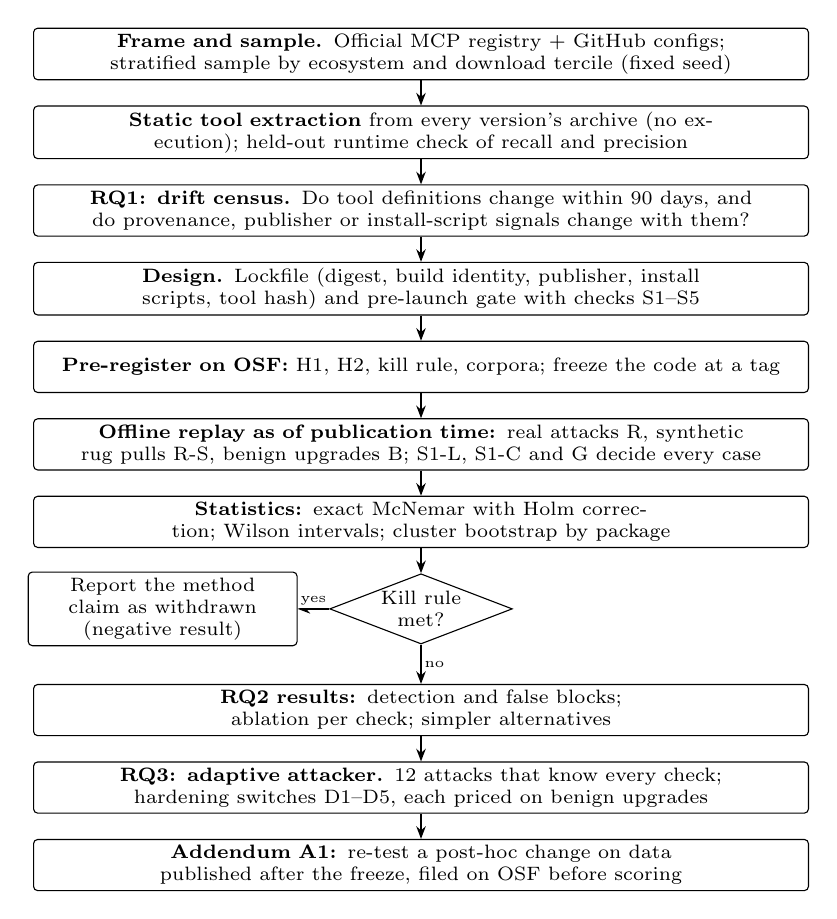
\begin{tikzpicture}[
  node distance=3.2mm,
  box/.style={draw, rounded corners=1.5pt, align=center, font=\scriptsize, minimum height=6.5mm,
              text width=0.80\columnwidth, inner sep=2pt},
  dec/.style={draw, diamond, aspect=2.6, align=center, font=\scriptsize, inner sep=0.5pt},
  side/.style={draw, rounded corners=1.5pt, align=center, font=\scriptsize, text width=0.27\columnwidth,
               inner sep=2pt},
  arr/.style={-{Stealth[length=1.6mm]}, semithick},
  lab/.style={font=\tiny, fill=white, inner sep=1pt}]
\node[box] (frame) {\textbf{Frame and sample.} Official MCP registry + GitHub configs; stratified sample by
  ecosystem and download tercile (fixed seed)};
\node[box, below=of frame] (extract) {\textbf{Static tool extraction} from every version's archive (no execution);
  held-out runtime check of recall and precision};
\node[box, below=of extract] (rq1) {\textbf{RQ1: drift census.} Do tool definitions change within 90 days, and do
  provenance, publisher or install-script signals change with them?};
\node[box, below=of rq1] (design) {\textbf{Design.} Lockfile (digest, build identity, publisher, install scripts,
  tool hash) and pre-launch gate with checks S1--S5};
\node[box, below=of design] (prereg) {\textbf{Pre-register on OSF:} H1, H2, kill rule, corpora; freeze the code at a
  tag};
\node[box, below=of prereg] (replay) {\textbf{Offline replay as of publication time:} real attacks R, synthetic rug
  pulls R-S, benign upgrades B; S1-L, S1-C and G decide every case};
\node[box, below=of replay] (stats) {\textbf{Statistics:} exact McNemar with Holm correction; Wilson intervals;
  cluster bootstrap by package};
\node[dec, below=of stats] (kill) {Kill rule\\met?};
\node[side, left=4mm of kill] (neg) {Report the method claim as withdrawn (negative result)};
\node[box, below=5mm of kill] (rq2) {\textbf{RQ2 results:} detection and false blocks; ablation per check;
  simpler alternatives};
\node[box, below=of rq2] (rq3) {\textbf{RQ3: adaptive attacker.} 12 attacks that know every check; hardening
  switches D1--D5, each priced on benign upgrades};
\node[box, below=of rq3] (a1) {\textbf{Addendum A1:} re-test a post-hoc change on data published after the freeze,
  filed on OSF before scoring};
\draw[arr] (frame) -- (extract);
\draw[arr] (extract) -- (rq1);
\draw[arr] (rq1) -- (design);
\draw[arr] (design) -- (prereg);
\draw[arr] (prereg) -- (replay);
\draw[arr] (replay) -- (stats);
\draw[arr] (stats) -- (kill);
\draw[arr] (kill) -- node[lab, above] {yes} (neg);
\draw[arr] (kill) -- node[lab, right] {no} (rq2);
\draw[arr] (rq2) -- (rq3);
\draw[arr] (rq3) -- (a1);
\end{tikzpicture}
\caption{Methodology. The census (RQ1) motivates the design; the evaluation (RQ2) is pre-registered with a kill
rule; the adaptive attacker (RQ3) and addendum A1 follow.}
\label{fig:method}
\end{figure}

\setcounter{section}{7}
% Performance comparison with existing methods. Every cell is a macro from numbers.tex.
\section{Comparison with Existing Methods}
\label{sec:compare}
Table~\ref{tab:compare} sets MCP-Lock beside both readings of the baseline hook and two measures that need no gate,
all on the corpora of Section~\ref{sec:eval}. On npm attacks, the hook combined with \code{-{}-ignore-scripts} reaches
roughly the detection of \G{} (\SCIgnP{} vs.\ \GNpmP), so a cheaper route to most of \G's real-attack gain exists. The
rug pulls separate them: the hook catches \RSSC{} and \G{} catches \RSG. Pinning an exact version stops \PinRMP{} of
R-M and, trivially, every rug pull, but every one of the \NB{} honest upgrades then waits until someone edits the
configuration. \G{} lets an upgrade through on its own when none of its checks sees a change.

\begin{table}[t]
\caption{Comparison with existing methods.\\
\textmd{R: real attacks ($n=\NR$); R-S: synthetic rug pulls; B: benign upgrades ($n=\NB$). The npm column uses the
npm cases of R-M. -- not applicable.}}
\label{tab:compare}
\centering
\footnotesize
\setlength{\tabcolsep}{2.5pt}
\resizebox{\columnwidth}{!}{%
\begin{tabular}{@{}lcccc@{}}
\toprule
Method & R detected & npm R-M & R-S & B false blocks \\
\midrule
Hook, literal (S1-L)~\cite{bagmar2026setup} & \DetSLP{} & -- & \RSSL{} & \FbSLP{} \\
Hook, charitable (S1-C) & \DetSCP{} & \SCNpmP{} & \RSSC{} & \FbSCP{} \\
Exact version pin & -- & -- & all$^{d}$ & all held back \\
\code{-{}-ignore-scripts} (npm) & -- & \IgnRMP{}$^{a}$ & -- & \IgnBP{}$^{b}$ \\
S1-C + \code{-{}-ignore-scripts} & -- & \SCIgnP{} & -- & -- \\
\textbf{MCP-Lock (\G)} & \textbf{\DetGP} & \GNpmP{} & \textbf{\RSG} & \FbGP{} \\
\G{}, locked servers exempt from age rule$^{c}$ & \AgeDetP{} & -- & -- & \AgeFbP{} \\
\bottomrule
\end{tabular}}

\vspace{2pt}
\begin{minipage}{\columnwidth}\scriptsize
$^{a}$Upper bound; a payload may also run at launch. $^{b}$npm upgrades whose honest install script would be skipped.
$^{c}$Exploratory; not confirmed on new data (\AoneLost{} of \AoneRC{} hijacked cases missed). $^{d}$A pinned launch
never runs a new version. Median gate latency: \LatColdMed{}\,s cold, \LatWarmMed{}\,s warm.
\end{minipage}
\end{table}

\bibliographystyle{IEEEtran}
\bibliography{refs}
\end{document}
